\newcommand{\e} {\`e }
\newcommand{\E} {\`E }
\newcommand{\aee} {\'{e} }
\newcommand{\aea} {\`{a} }
\newcommand{\ai} {\`{\i} }
\newcommand{\ao} {\`{o} }
\newcommand{\au} {\`{u} }
\newcommand{\bit} {\begin{itemize} }
\newcommand{\eit} {\end{itemize} }


%\documentclass[handout]{beamer}
\documentclass{beamer}
\usepackage{pgfpages}
\usepackage{graphicx}
\usepackage{multicol}
\usepackage{caption}
\usepackage{makecell}
%\pgfpagesuselayout{2 on 1}[a4paper, border shrink=5mm]

\usepackage{helvet}
\renewcommand{\familydefault}{\sfdefault}

\usepackage{listings}
\usepackage{xcolor}

\definecolor{UNIFIblue}{rgb}{0, 0.298, 0.494	}  

\usecolortheme[named=UNIFIblue]{structure}

%\usetheme{PaloAlto}
\usetheme{Pittsburgh}
%\usetheme{Berkeley}


\definecolor{White}{rgb}{1.0,1.0,1.0}
\definecolor{Blue}{rgb}{0.,0.,1.}
\definecolor{Pink}{rgb}{1.,0.75,0.8}
\definecolor{LRed}{rgb}{1.0,0.2,0.2}
\definecolor{Red}{rgb}{1.0,0.0,0.0}

\beamertemplatenavigationsymbolsempty

\setbeamertemplate{background}
{
\includegraphics[width=\paperwidth,height=\paperheight,keepaspectratio]{Immagine1}}
 



\begin{document}
\title{\textcolor{White}{Parallel Image Composition}}  
\author{\textcolor{White}{Nicol\ao Pollini, Francesco Fantechi}}
\date{\textcolor{White}{A.A. 2022-2023}}
 

 
\frame{\titlepage} 

%%%%%%%%%%%%%%%%%%%%%%%%%%%%%%%%%%%%%%%%%%%%%%%%%%%%%%%%%%%%%%%%%%%%%%%%%

%%%%%%%%%%%%%%%%%%%%%%%%%%%%%%%%%%%%%%%%%%%%%%%%%%%%%%%%%%%%%%%%%%%%%%%%%
\setbeamertemplate{background}
{
\includegraphics[width=\paperwidth,height=\paperheight,keepaspectratio]{Immagine2}}





 
 
 \frame{\frametitle{Indice}
 \tableofcontents
 } 
 
 
 
 
 
 \setbeamercolor{date in head/foot}{fg=White, bg=UNIFIblue}
 \setbeamertemplate{footline}
 {
 	\begin{beamercolorbox}[ht=1ex,sep=1ex, center]{date in head/foot}
 		\insertshorttitle \ \ \hspace{2cm}  \insertsection  \ \ \ \insertsubsection \hfill\insertframenumber%/\inserttotalframenumber
 	\end{beamercolorbox}
 	
 }
 
 
 %%%%%%%%%%%%%%%%% PARTI DA QUI CON I TUOI FRAME!!!! %%%%%%%%%%%%%%%%%%%%%%%
 
 
 \section{Obiettivo}
 
 \frame{\frametitle{Obiettivo}
 	
	\bit
	\item {\color{Blue} Parallelizzare un algoritmo di Data
Augmentation che effettua composizioni di immagini}
\item{\color{Blue} Utilizzando:}
	\bit
	\item {\color{Blue} Framework OpenMP}
	\item {\color{Blue} Librerie Python che permettono il multiprocessing}
	\eit
	\item {\color{Blue} Confrontare i vari
metodi valutando gli speedup ottenuti rispetto alle loro esecuzioni sequenziali}
	\begin{figure}
	\flushleft
	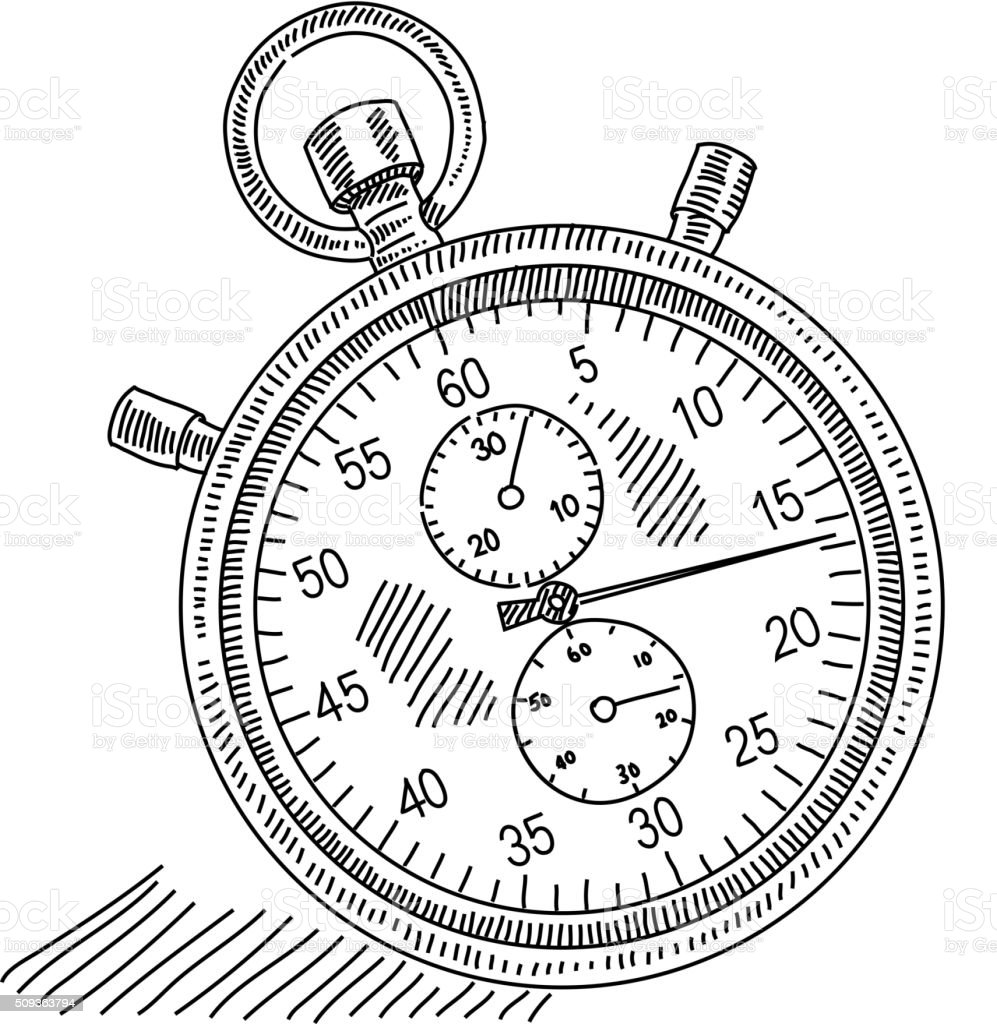
\includegraphics[width=0.2\textwidth]{Immagini/Cronometro}
	\end{figure}
	\centering
	\eit	
 	
 	
 }
 
 \section{Data Augmentation}
 
 \frame{\frametitle{Data Augmentation}
 	
	\bit
	\item {\color{Blue} Insieme di processi atti ad aumentare gli elementi
di un dataset senza raccogliere nuovi dati}
\item{\color{Blue} Tecnica che trova un largo impiego
nell’addestramento delle reti neurali quando i dati a disposizione non sono nu-
mericamente sufficienti}
	\begin{figure}
	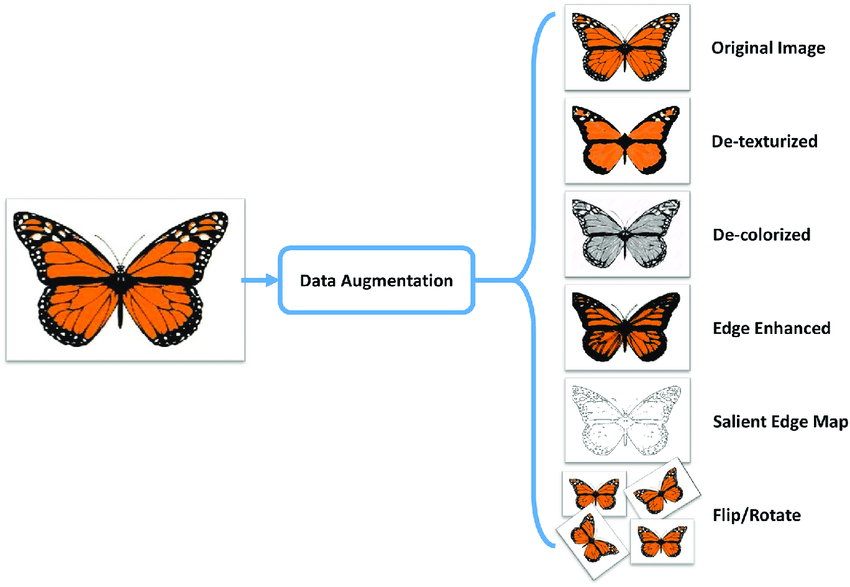
\includegraphics[width=0.6\textwidth]{Immagini/DataAugmentation}
	\end{figure}
	\eit	
 	
 	
 }
 
 \subsection{Image Composition}
 
 \frame{\frametitle{Image Composition}
 	
	\bit
	\item[] {\color{Blue} Nel nostro esperimento:}
	\bit
\item{\color{Blue} Dataset: $ 5 $ immagini di background di dimensione
$483\times594$ pixel raffiguaranti dei quokka}
\item{\color{Blue} Data Augmentation: mediante Image Composition applicando un’ulteriore immagine di dimensione 298 × 350
pixel}
\eit
	\begin{figure}
	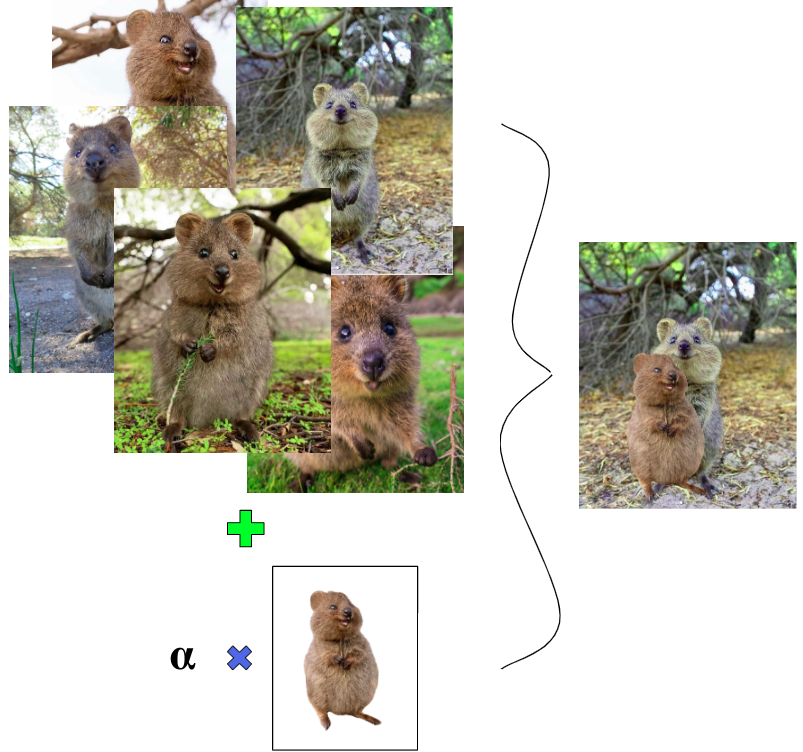
\includegraphics[width=0.45\textwidth]{Immagini/Images}
	\end{figure}
	\eit	
 	
 	
 }



\section{Codice e implementazione}

\frame{\frametitle{Codice e implementazione}
	
	
	\bit
	\item {\color{Blue} Progetto implementato in linguaggio C++ e Python}
	\item{\color{Blue} Codice versionato tramite la piattaforma GitHub:}
	\bit
	\item[] { \tiny - \url{https://github.com/francesco-ftk/Image_Composition_OpenMP.git}}
\item[] {\tiny - \url{https://github.com/francesco-ftk/Image_Composition_Multiprocessing.git}}
\eit
	\item {\color{Blue} Eseguito su due diverse macchine con due diversi OS: }
	\begin{figure}
	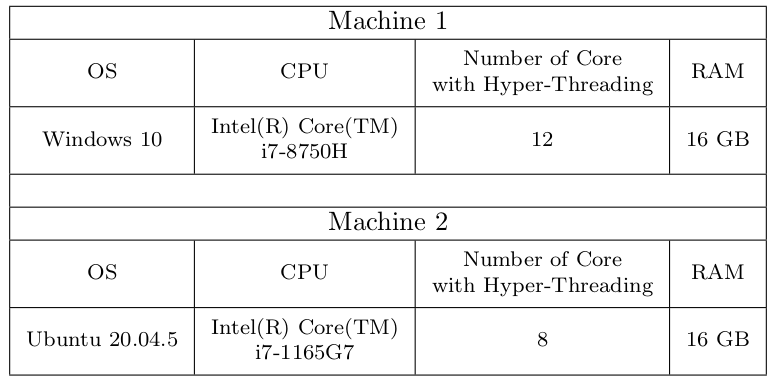
\includegraphics[width=0.7\textwidth]{Immagini/Macchine}
	\end{figure}
	\eit
	
}


\frame{\frametitle{Codice e implementazione}
	
	\bit
	\item {\color{Blue} Il progetto \e stato suddiviso in tre parti:}
	\bit
		\item {\color{Blue} Implemenatazione dell’agoritmo di Image Composition sequenziale}
		\item {\color{Blue} Parallelizzazione dell’algoritmo tramite il framework OpenMP in C++}
		\item {\color{Blue} Parallelizzazione dell’algoritmo tramite le librerie di multiprocessing in Python}
	\eit
	\eit
	
	
}

\subsection{Image Composition Sequenziale}

\frame{\frametitle{Image Composition Sequenziale}
	
	\bit
	\item {\color{Blue} Parametro \textit{“transformations”} indicativo del numero di nuove immagini volute}
	\item {\color{Blue} Per \textit{“transformations”} volte:}
	\bit
		\item {\color{Blue} Presa un’immagine fra quelle possibili di
background in modo randomico}
		\item {\color{Blue} Aggiunta in posiszione randomica l'immagine di foreground con una trasparenza uniformemente scelta nell'intervallo $ [128,255] $}
		\item {\color{Blue} Immagini lette, editate e salvate tramite la libreria OpenCV}
	\eit
	\eit
}

\frame{\frametitle{Estratto Codice Python}
	\bit
	\item[] {\color{Blue} \small Image Composition Sequenziale}
	\vspace{5px}
	\begin{figure}
	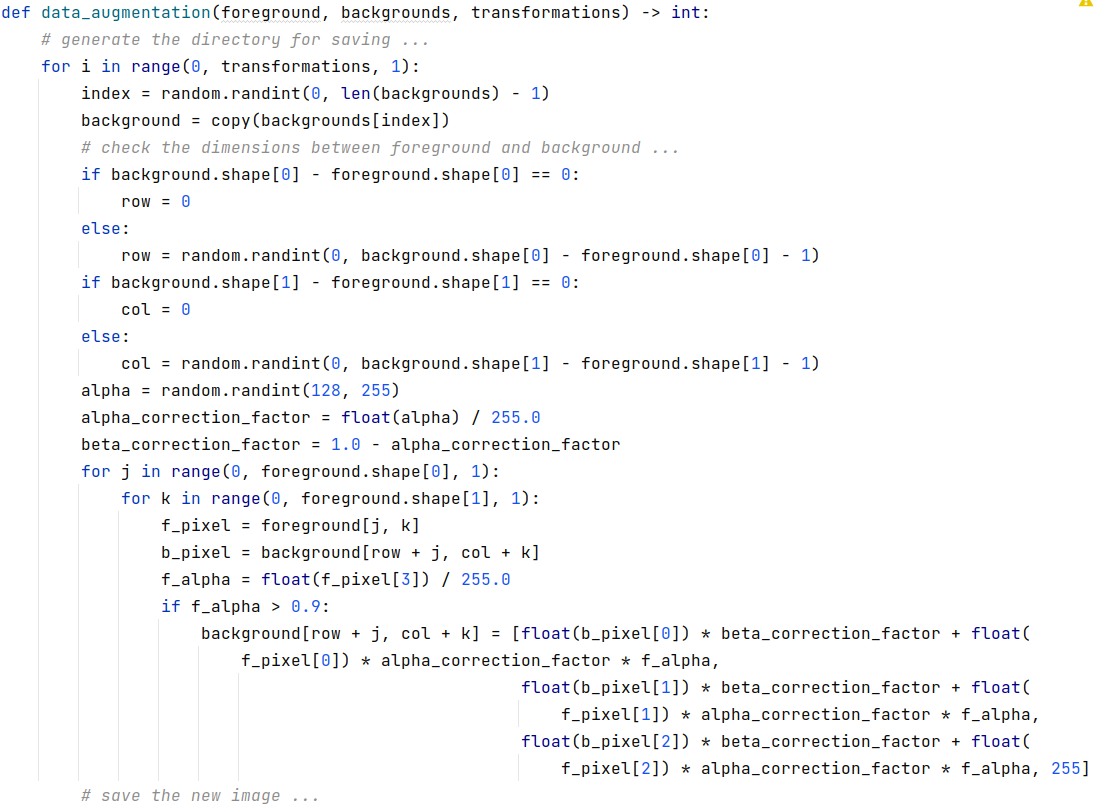
\includegraphics[width=0.7\textwidth]{Immagini/Sequential}
	\end{figure}
	\eit
}

\subsection{OpenMP}

\frame{\frametitle{OpenMP}
	
	\bit
	\item {\color{Red} Framework OpenMP}
	\item {\color{Blue} Permette di parallelizzare una porzione di codice in modalit\aea implicit threading attraverso delle direttive “pragma”}
	\item {\color{Blue} Ogni thread genera una porzione delle immagini di output richieste tramite il parametro \textit{“transformations”}}
	\item {\color{Blue} Algoritmo imbarazzantemente parallelo}
	\item {\color{Blue} Numero di thread usati calcolato aggiungendo un
$50\%$ al numero complessivo di Core posseduti dalla macchina utilizzata considerando l’Hyper-Threading}
	\eit
}

\frame{\frametitle{Estratto Codice C++}
	\bit
	\item[] {\color{Blue} \small OpenMP}
	\begin{figure}
	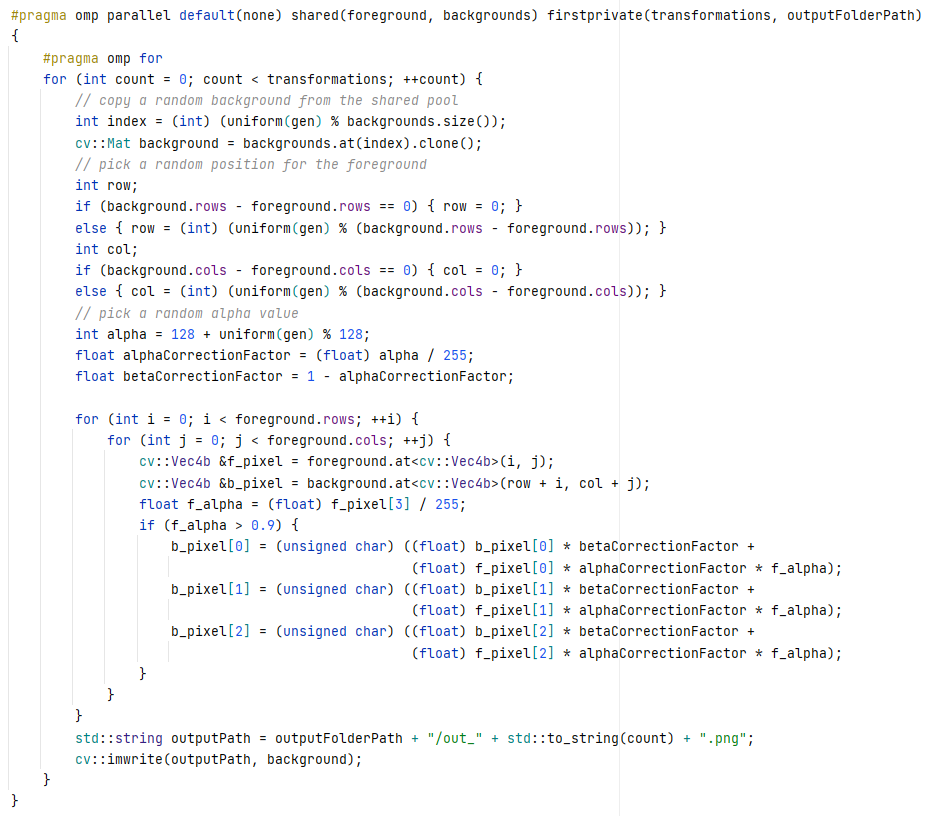
\includegraphics[width=0.7\textwidth]{Immagini/OpenMP}
	\end{figure}
	\eit
}

\subsection{Multiprocessing}

\frame{\frametitle{Multiprocessing}
	
	\bit
	\item {\color{Blue} Interprete Python GIL (Global Interpretr Lock)}
	\item {\color{Blue} In Python non \e possibile eseguire piú di un thread contemporaneamente}
	\item {\color{Red} $ \rightarrow $ Sottoprocessi al posto dei thread}
	\item {\color{Blue} Molto piú costosi rispetto a far partire dei thread}
	\item {\color{Blue} Due metodi differenti per istanziare i sottoprocessi:}
	\bit
	\item {\color{Blue} Libreria standard di Python Multiprocessing}
	\item {\color{Blue} Libreria Joblib}
	\eit
	\item{\color{Blue} Numero di processi istanziati calcolato aggiungendo un $50\%$ al numero complessivo di Core posseduti dalla macchina utilizzata considerando l’Hyper-Threading}
	\eit
}

\frame{\frametitle{Multiprocessing}
	
	\bit
	\item {\color{Red} Libreria Multiprocessing}
	\item {\color{Blue} Permette di istanziare e far partire manualmente i processi su una certa funzione target}
	\item {\color{Blue} Lavoro equamente diviso fra i vari processi}
	\item {\color{Blue} Parametro \textit{“transformations\_for\_process”} ottenuto dividendo il numero di nuove immagini volute per il numero di processi istanziati}
	\item {\color{Blue} Due implementazioni equivalenti del suo utilizzo implementate:}
	\bit
	\item {\color{Blue} Multiprocessing}
	\item {\color{Blue} Multiprocessing con Pooling}
	\eit
	\eit
}

\frame{\frametitle{Estratto Codice Python}
	\bit
	\item[] {\color{Blue} Multiprocessing}
	\vspace{15px}
	\begin{figure}
	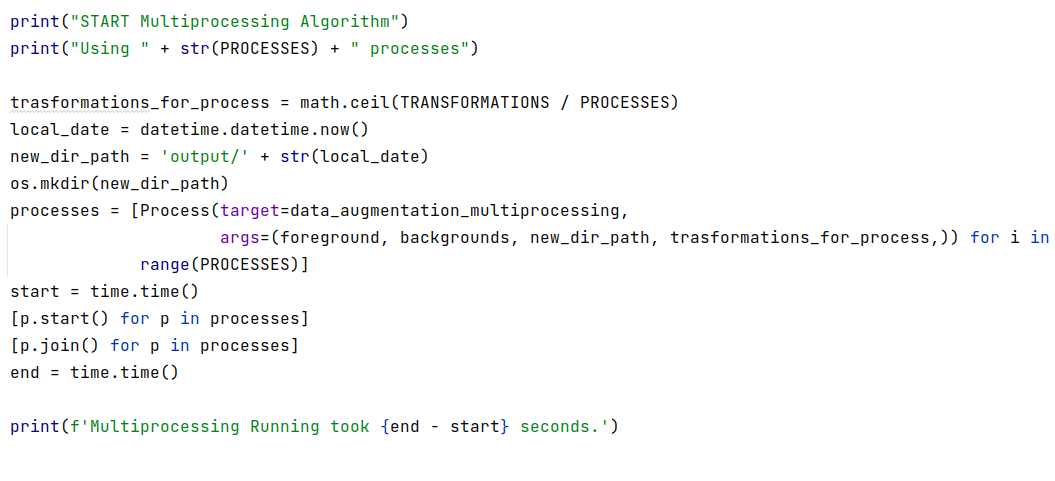
\includegraphics[width=0.9\textwidth]{Immagini/Multiprocessing}
	\end{figure}
	\eit
}

\frame{\frametitle{Estratto Codice Python}
	\bit
	\item[] {\color{Blue} Pooling Multiprocessing}
	\vspace{5px}
	\begin{figure}
	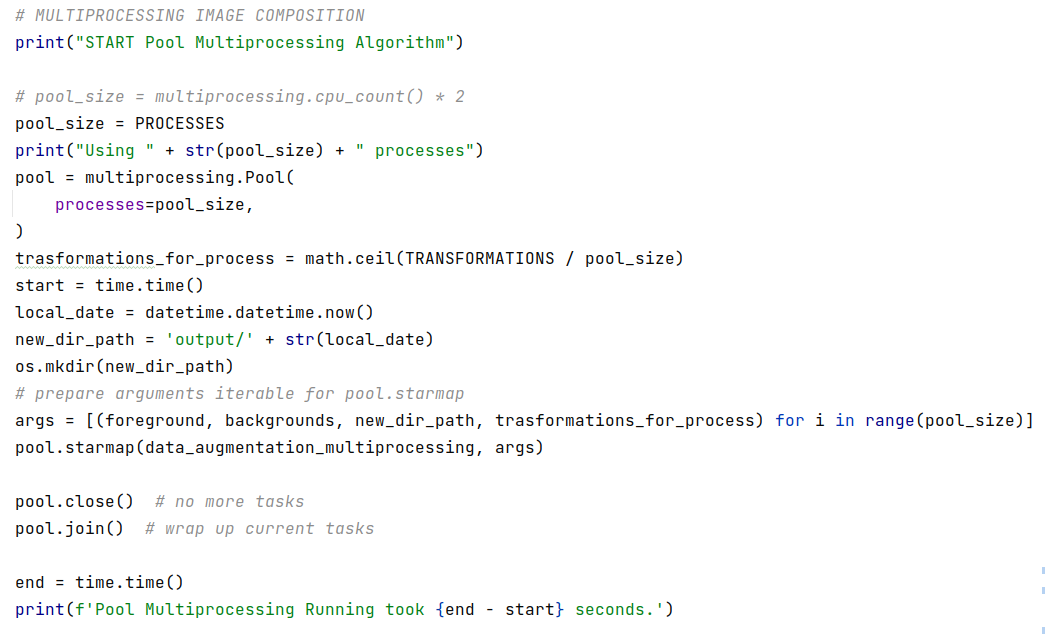
\includegraphics[width=0.9\textwidth]{Immagini/Pool}
	\end{figure}
	\eit
}

\frame{\frametitle{Joblib}
	
	\bit
	\item {\color{Red} Libreria Joblib}
	\item {\color{Blue} Processi eseguiti in modo asincrono sulla propria funzione target suddividendosi il lavoro in modo autonomo}
	\item {\color{Blue} Ad ogni nuova esecuzione di un processo gli argomenti posseduti devono essere ripassati in ingresso alla funzione}
	\item {\color{Blue} Per ridurre i costi ogni processo genera una nuova immagine alla volta e riceve gi\aea negli argomenti l'immagine di background da utilizzare e non l'intero dataset da cui scegliere}
	\eit
}

\frame{\frametitle{Estratto Codice Python}
	\bit
	\item[] {\color{Blue} Joblib}
	\vspace{5px}
	\begin{figure}
	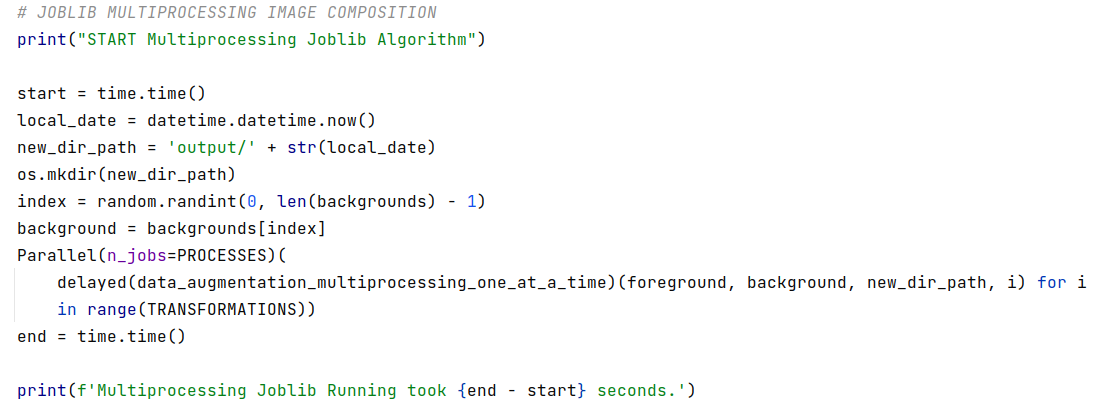
\includegraphics[width=0.9\textwidth]{Immagini/Joblib}
	\end{figure}
	\eit
}

\section{Risultati}

\frame{\frametitle{Risultati C++}
	\bit
	\item[] {\color{Blue} \small Timing OpenMP Macchina $ 1 $ al variare del numero dei thread}
	\vspace{5px}
	\begin{figure}
	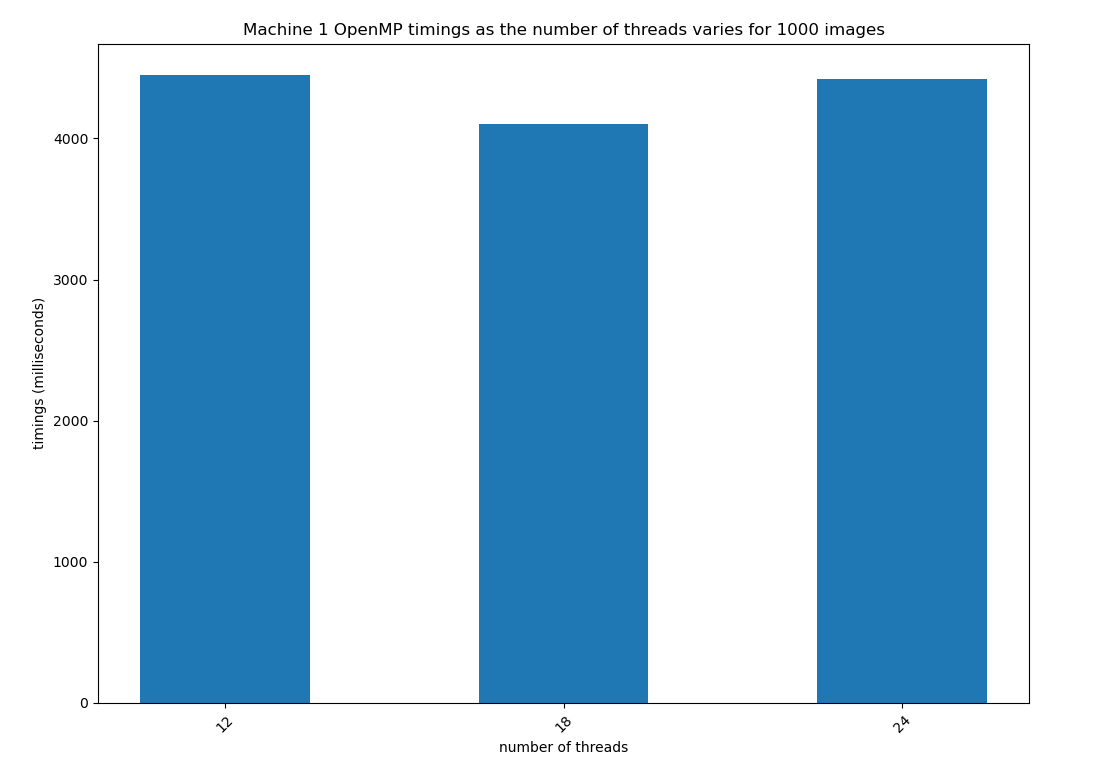
\includegraphics[width=0.8\textwidth]{Immagini/Timings_Varying_Threads}
	\end{figure}
	\eit
}

\frame{\frametitle{Risultati C++}
	\bit
	\item[] {\color{Blue} \small Timings e Speedup Macchina $1$ OpenMP}
	\bit
		\item {\color{Blue} $18$ thread}
	\eit
	\begin{center}
	\captionof{table}{\color{Blue} C++ Timings}
\begin{tabular}{|c|c|c|}
\hline
\multicolumn{3}{|c|}{Machine 1}\\
\hline
\thead{Number of Images} & \thead{Sequential} & \thead{OpenMP} \\
\hline
\thead{$ 1800 $} & \thead{$ 88974ms $} & \thead{$ 14832ms $}\\
\hline
\end{tabular}
\vspace{5px}
\captionof{table}{\color{Blue} Speedups}
\begin{tabular}{|c|c|c|c|}
\hline
\multicolumn{4}{|c|}{Machine 1}\\
\hline
\multicolumn{4}{|c|}{OpenMP}\\
\hline
\multicolumn{4}{|c|}{$ 6.0 $}\\
\hline
\end{tabular}
\end{center}
	\eit
}

\frame{\frametitle{Risultati C++}
	\bit
	\item[] {\color{Blue} \small Speedup OpenMP Macchina $ 1 $ al variare del numero di immagini generate con $18$ thread}
	\vspace{5px}
	\begin{figure}
	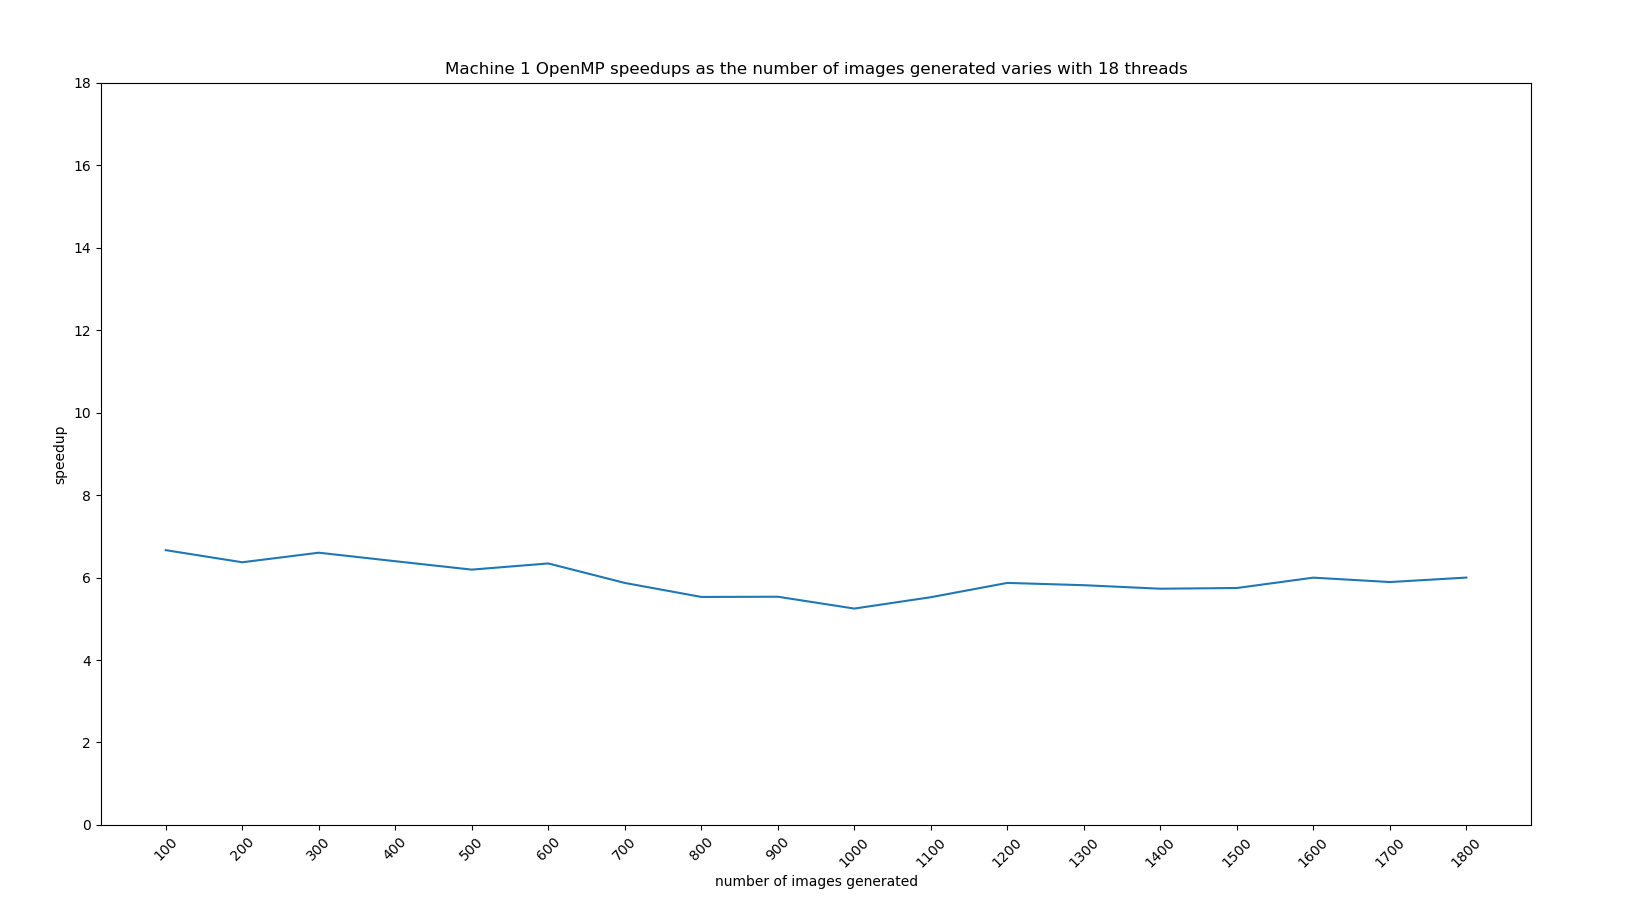
\includegraphics[width=0.9\textwidth]{Immagini/Speedup_Varying_Transformations}
	\end{figure}
	\eit
}

\frame{\frametitle{Risultati Python}
	\bit
	\item[] {\color{Blue} \small Timings e Speedup Macchina $2$ Multiprocessing}
	\bit
		\item {\color{Blue} $12$ processi}
	\eit
\captionof{table}{\color{Blue} Python Timings}
\hspace{-22px}\begin{tabular}{|c|c|c|c|c|}
\hline
\multicolumn{5}{|c|}{Machine 2}\\
\hline
\thead{Number of Images} & \thead{Sequential} & \thead{Joblib} & \thead{Pool Multiprocessing} & \thead{Multiprocessing} \\
\hline
\thead{$ 1200 $} & \thead{$ 122.1s $} & \thead{$ 143.9s $} & \thead{$ 52.1s $}  & \thead{$ 50.7s $}\\
\hline
\end{tabular}
\vspace{5px}
\begin{center}
\captionof{table}{\color{Blue} Speedups}
\begin{tabular}{|c|c|c|c|} 
\hline
\multicolumn{4}{|c|}{Machine 2}\\
\hline
\multicolumn{1}{|c|}{\hspace*{0.5cm}Joblib\hspace*{0.5cm}} & \multicolumn{2}{c|}{Pool Multiprocessing} & \multicolumn{1}{c|}{Multiprocessing}\\
\hline
\multicolumn{1}{|c|}{$ 0.9 $} & \multicolumn{2}{c|}{$ 2.3 $} & \multicolumn{1}{c|}{$ 2.4 $}\\
\hline
\end{tabular}
\end{center}
	\eit
}

\frame{\frametitle{Risultati Python}
	\bit
	\item[] {\color{Blue} \small Speedup Multiprocessing Macchina $ 2 $ al variare del numero di immagini generate con $12$ processi}
	\vspace{5px}
	\begin{figure}
	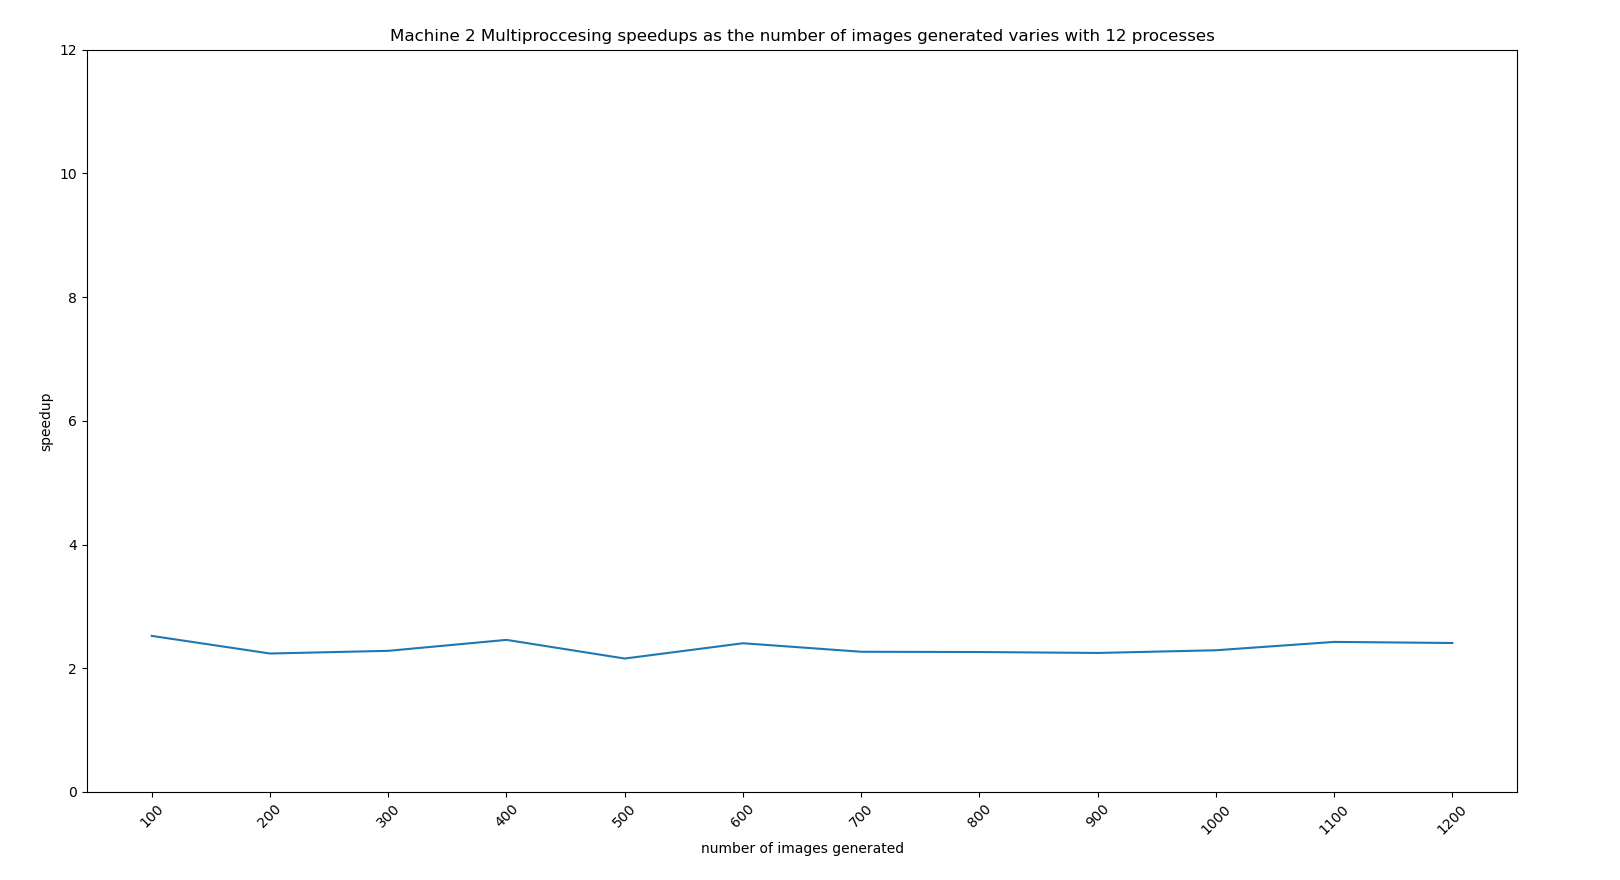
\includegraphics[width=0.9\textwidth]{Immagini/Speedup_Varying_Transformations_Multiprocessing}
	\end{figure}
	\eit
}

\section{Conclusioni}

\frame{\frametitle{Conclusioni}
	
	\bit
	\item {\color{Blue} Speedup sublineare sia con OpenMP che con la libreria Multiprocessing}
	\item {\color{Blue} Speedup con la libreria Multiprocessing nettamente inferiore a quello ottenuto con OpenMP}
	\item {\color{Blue} Nessuno speedup tramite l'utilizzo della libreria Joblib}
	\eit
}


\end{document}
